\section{Геометрические задачи}

\subsection{Площадь сферического треугольника}
\begin{center}
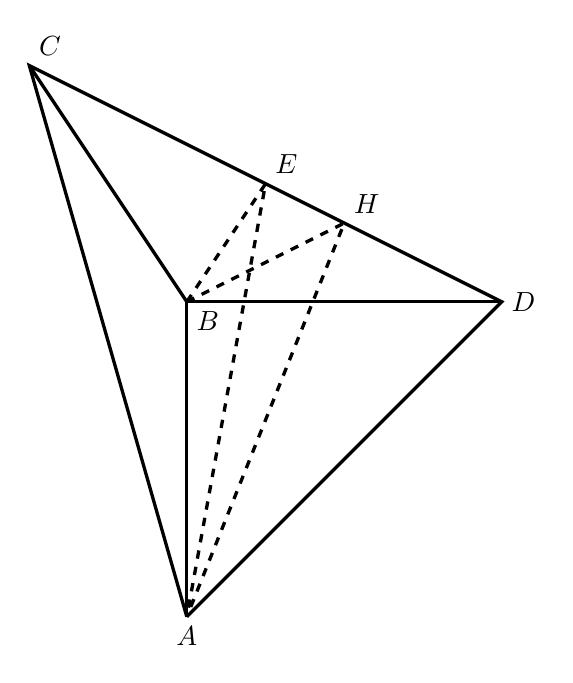
\begin{tikzpicture}
\coordinate (B) at (0, 0);
\coordinate (D) at (4, 0);
\coordinate (C) at (-2, 3);
\coordinate (E) at (1, 1.5);
\coordinate (H) at (2, 1);
\coordinate (A) at (0, -4);

\draw[very thick] (A) -- (C) -- (D) -- (A);
\draw[very thick] (B) -- (A);
\draw[very thick] (B) -- (C);
\draw[very thick] (B) -- (D);
\draw[very thick, dashed] (B) -- (H) -- (A);
\draw[very thick, dashed] (B) -- (E) -- (A);

\draw (B) node[below right] {$B$};
\draw (D) node[right] {$D$};
\draw (C) node[above right] {$C$};
\draw (H) node[above right] {$H$};
\draw (E) node[above right] {$E$};
\draw (A) node[below] {$A$};
%\draw [fill=black] (0.,1.) circle (2.5pt);
\end{tikzpicture}	
\end{center}

Здесь у нас $\angle ABC = 90^\circ$, $\angle ABD = 90 ^\circ$, $\angle BHD = 90^\circ$. Дальше будем использовать обозначения: $\angle BAH = \theta_h$, $\angle BAC = \alpha$, $\angle BAD = \beta$, $\angle CAD = \gamma$, $\angle BAE = \theta$, $\angle HBE = \varphi$, $\angle HBC = \varphi_\alpha$, $\angle HBD = \varphi_\beta$, $\angle CBD = \Phi$. Наша задача найти интеграл
\[
	\int \sin \theta d\theta d\varphi = \int\limits_{-\varphi_\alpha}^{\varphi_\beta} (1 - \cos(\theta(\varphi))) d\varphi
\]
\[
	\frac{BE}{AB} = \tan \theta \quad
	\frac{BH}{BE} = \cos \varphi \quad
	\frac{BH}{AB} = \tan \theta_h
\]
\[
	\tan \theta \cos \varphi = \tan \theta_h
\]
\[
	\cos \theta = \frac{1}{\sqrt{1 + \left(\frac{\tan \theta_h}{\cos \varphi}\right)^2}} 
	=
	\frac{\cos \varphi}{\sqrt{1 + \frac{\cos^2 \varphi}{\tan^2 \theta_h}}} \frac{1}{\tan \theta_h}
	=
	\frac{\cos \varphi}{\sqrt{\frac{1}{\cos^2 \theta_h} - \sin^2 \varphi}} =
	\frac{\cos \theta_h \cos \varphi}{\sqrt{1 - \cos^2 \theta_h \sin^2 \varphi}}
\]
\[
	\int \sin \theta d\theta d\varphi = \Phi - \arcsin (\cos \theta_h \sin \varphi_\alpha) - \arcsin (\cos \theta_h \sin \varphi_\beta)
\]
